%!TEX root = main.tex
\subsection{Introduction}

Lexical semantics focus on the meaning of words. We call \textbf{lexeme} a pair of \textit{form} with its \textit{meaning}. A lexeme is represented by a \textbf{lemma}. The meaning of a lema can vary given the context. \\
A \textbf{word sense} is a discrete representatin of one aspect of the meaning of the word. If two senses from a same word have no semantic relation, they are \textbf{homonyms}. Else its \textbf{polysemy} (ex. \textit{mouse}). If two senses are related, they are viewed as two senses of a \textbf{polysemous lexeme}. A kind of polysemy is \textbf{metonomy}, where we replace an aspect of a concept by the concept (ex. \textit{boire un verre}).

\subsection{Relation between senses}

\subsubsection{Synonymy and antonymy}

Two words are \textbf{synonyms} if they are substituable one for the other in any sentence without changing the truth condition of the sentence. \textbf{Antonymy} is more complex to define because two senses can be antonyms in many ways:
\begin{itemize}
 	\item \textbf{Binary opposition}: alive/dead; true/false;
 	\item \textbf{Opposite ends of some scale}: cold/warm; rapid/slow;
 	\item \textbf{Reversive}: rize/fall; up/down; buy/sell.
 \end{itemize} 

 Better to describe synonymy as a relation between senses (ex \textit{hot - spicy}). Hard to automatize a task to distinguish synonyms to antonyms. 

\subsubsection{Hierarchical relations}

One sense is a \textbf{hyponym} of another sense if the first sense is more specific, denoting a subclass. \textit{Cat} is hyponym of \textit{animal}. A \textbf{hypernym} is the inverse. \\

A \textbf{taxonomy} is a collection of controlled vocabulary terms organized into a hierarchical structure. Each term in a taxonomy is in one or more parent-child relationships to other terms in the taxonomy. A \textbf{thesaurus} is a networked collection of controlled vocabulary terms. This means that a thesaurus uses associative relationships in addition to parent-child relationships. An \textbf{ontology} is an explicit and formal specification of a conceptualization (Gruber 1993). It uses a controlled vocabulary.

\subsection{Three approaches to lexical semantics}

\subsubsection{Lexical relations}

Relations between the senses of words. \textbf{WordNet} is a lexical database accessible through word senses. There are three databases: one for nouns, one for verbs and one for adjectives and adverbs. A \textbf{synset} is a set of equivalent synonyms. A \textbf{glose} describe the concept heind the synset.

\subsubsection{Event participation}

\textbf{Thematic roles} are an attempt to categorize commonality of different roles (agent, experiencer, force, theme, result, \dots). The benefit is to allows simple inferences with a shallow meaning representation. The problem: difficult to standardize and formalize roles.

\paragraph{PropBank}

Annoted sentences with semantic roles (for verbs). Can use Treebank annotation.

\paragraph{FrameNet}

Based on \textbf{frames} (script-like structure that describes events).

\subsubsection{Selectional restrictions}

\textbf{Selectional Restrictions} express a kind of semantic constraint that a verb imposes on the kind of concepts that are allowed to fill its argument roles. We can use synset of WordNet to achieve this.

\subsection{Computational lexical semantics}

\subsubsection{Word sense disambiguation}

The goal is to select the sense for a given word in a given context. There is two tasks:
\begin{itemize}
	\item \textbf{Lexical sample task}: Only for a limited sample of words. Classifiers can be trained on hand labeled corpora;
	\item \textbf{All-words tasks}: Need other approaches due to sparseness/too much work for labeling by hand.
\end{itemize}

\newpage

\paragraph{Supervised WSD}

\subparagraph{Feature extraction}

The first step is to extract features that can help to predict word senses. We can use preprocess (POST, syntax, lemmatization, \dots). Then two classes of features can be used:

\begin{itemize}
	\item \textbf{Collectional features}: encode informations about specific positions at the left or right of the target word ([wi-2, POS i-2, wi-1, POS i-1, wi+1, POS i+1, wi+2 POS i+2], [guitar, NN, and, CC, player, NN, stand, VB]);
	\item \textbf{Bag od words features}: Unordred set of words in the context of the target word ([fishing,big,sound,player,fly,rod,pound,double,runs,playing,guitar,band], [0,0,0,1,0,0,0,0,0,0,1,0]).
\end{itemize}



\subparagraph{Bayesian approach}

Choosing the best sense $\hat{s}$ out of a set of possible senses $S$ for a feature vector $\vec{f}$ amounts to choosing the most probable sense given that vector.
$$\hat{s} = argmax_{s \in S} P(s|\vec{f}) = argmax_{s \in S} \frac{P(\vec{f}|s)P(s)}{P(\vec{f})}$$

Problem: not enough data to resolve this problem (20 words = $2^{20}$ vectors).

\subparagraph{Naive Bayes approach}

With the independence assumption: $P(\vec{f}|s) \approx \prod^{n}_{j=1} P(\vec{f_j}|s)$ we have $\hat{s} = argmax_{s \in S} P(s) \prod^{n}_{j=1} P(f_j|s)$. $P(s_i) = \frac{count(s_i , w_j)}{count(w_j)}$ and $P(f_j|s) = \frac{count(f_j, s)}{count(s)}$. Need smoothing.

\subparagraph{Dictionnary and Thesaurus method}

Hand-labelled corpora is not always available. A dictionary or thesaurus can provide an indirect kind of supervision. We select the sense from the lexical resources whose definition share the most words with the target word's neighborhood.

\begin{figure}[H]
	\centering
	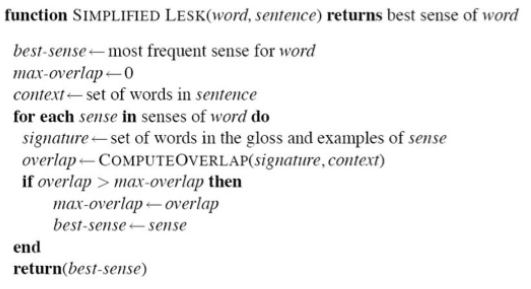
\includegraphics[scale=0.6]{images/68_lesk.png}
 	\caption{Lesk algorithm. Improvements: extend list of words used in classifier and use weighting: inverse document frequency $idf_{i} = log (\frac{Ndoc}{nd_{w_{i}}})$. Ndoc is the total number of definitions and $nd_{w_{i}}$ is the number of definitions which contains the word $w_{i}$.}
\end{figure}

\paragraph{WSD Evaluation}

Two ways to evaluate a WSD system: \textbf{task-based evaluation} (bad because the final application does not only depend of the WSD system) and \textbf{intrinsic evaluation} (percentage of correctness). We can use two different metrics: \textbf{baseline} (compared with first sense in WordNet) and \textbf{ceiling} (human inter annotator agreement). We can used two kinds of data: \textbf{hand labelled corpora} (supervised) and \textbf{pseudowords} (concatenation of two words, the WSD system must find the correct sense).

\subsubsection{Word similarity}

Kind of distance between words. There is two classes of algorithms:
\begin{itemize}
	\item \textbf{Thesaurus based method}: $sim_{path}(c_1 , c_2) = - log (pathlen(c_1 ,c_2))$;
	\item \textbf{Distributional approach}: find words with the same distribution in the context.
\end{itemize}

Note: theoretical distinction between word similaritiy and word relatedness (ex. \textit{car} and \textit{gasoline}). 